\documentclass[12pt,upcase]{mitthesis}

\usepackage{amsmath}
\usepackage{microtype}
\usepackage{graphicx}
\graphicspath{{./images/}}
\usepackage{multirow}
\usepackage{rotating}
\usepackage{natbib}
\usepackage{url}
\usepackage{booktabs}
\usepackage{minted}
\usepackage{scrextend}						% for the labelling list environment used in Ch4
\addtokomafont{labelinglabel}{\sffamily}	% for the labelling list environment used in Ch4

\usepackage[]{pdfpages}

% use fancyhdr, to enable page style stuff (below)
\usepackage{fancyhdr}
\setlength{\headheight}{15.2pt}
\renewcommand{\headrulewidth}{0pt}

\pagestyle{plain}

\begin{document}
\include{cover}
\chapter*{Acknowledgments}
\renewcommand{\thefootnote}{\fnsymbol{footnote}}

%TODO thank fred and committee

% It is common courtesy to seek permission before listing a person in acknowledgments, so that should be done for all. TODO
Special thanks to Derrell Lipman, Farzeen Harunani, Michael Tissenbaum, Drew Ditto, Kim Douglas, Molly Laden, Akira Kamiya, Ben Shapiro, Josh Sheldon, Hal Abelson, Mark Guzdial, Sally Fincher, and Benjamin Xie for their help throughout this work.

Thank you to my system testers, listed in full in the Appendix.

%Thank you to my system testers: Mike Staub, William Sokolowsky, Jr., Ambarish Roy, Justin Richer, Charles Kaneb, Nicholas McKinnon, Christian Quale, Joshua O. Carlson, Russell Bernstein, Alistair Stead, Peter Galvin, Jessica Spink, Tim Baird, Barry Sherman, Emily Jackson, Reed Spool, Caroline Fonseca, Jessica West, Christopher Rogacz, Marybeth Moriarty, Matthew Sherman, and Andrew Chanler.

Special thanks to Ashely Hale, the undergraduate research assistant who did a huge amount of the manual data coding. The analysis would not have been possible without her.

Thank you to my committee--- Lyn helped me lay the groundwork years ago, and continues to drive me towards what has become our common mission. Jay helped steer the work towards its logical conclusion, and I am grateful for his enthusiasm and his eye for structure. Of course, I offer the deepest gratitude to my thesis supervisor and long-time advisor, Fred Martin. Fred first inspired me to pursue my casual interest in education, and taught me how to focus and hone that into a passion, mission, and career. Thank you, Fred. 

I would especially like to thank all my friends and family who have helped me stay strong. Thank you, Michelle Dubuke, my thesis buddy.

Finally, to my wife Stacy, thank you for your endless love and support. I could not have done this without you.

%TODO thank stacy, family, friends (Michelle, )

This material is based upon work supported by the National Science Foundation under Grants DUE-1225719 and DRL-1433592.\footnote{Any opinions, findings, and conclusions or recommendations expressed in this material are those of the author and do not necessarily reflect the views of the National Science Foundation.}

\renewcommand{\thefootnote}{\arabic{footnote}}
\include{contents}
%\include{preface} 	% Preface is not part of the standard. I invented it for myself. Use it if you want by uncommenting.

	% Redefine the "plain" pagestyle to have pagenum in the header, right
	\fancypagestyle{plain}{
		\fancyhf{}
		\fancyhead[R]{\thepage}
	}

	\setcounter{page}{1}
	\pagenumbering{arabic}
	\pagestyle{plain}
	
\chapter{Introduction}

\section{Research Focus}
 
\section{Problem Statement} \label{sec:problem-statement}

In February of 2015, nearly two years ago, the research question was simple, ``What questions could be answered if App Inventor were instrumented?'' Today we have such a set of questions, concentrated in three classes, concerning the construction of that instrumentation, the data that it would produce, and finally, the nature of blocks programming to which it provides access. The primary question, to which all the other questions are effectively in service, is:

\begin{quote}
\textbf{Does a pattern of block movement or manipulation exist that signals that the student is not working productively?}
\end{quote}

This question asks about \emph{flailing,} a behavior of making unproductive, sometimes random changes to the code, possibly elicited by the student being lost, and requires teacher intervention. A thorough discussion of flailing and other behaviors will follow in Section \ref{sec:behaviors}.

The complete set of research questions is below, with classes presented in ascending order of research importance:

\begin{enumerate}
\item Questions Concerning the Construction of a Distributed Snapshot System

\begin{enumerate}
\item \label{RQ:1.1} How can a system be built to snapshot blocks-based programming in App Inventor? 
\item \label{RQ:1.2} How can captured snapshot data from ephemeral, remote user sessions be securely and consistently housed in a central server? 
\item \label{RQ:1.3} What is the correct degree of granularity for such snapshot data?
\item \label{RQ:1.4} What actions by the user in the graphical, blocks-based system are appropriate to trigger a snapshot?
\item \label{RQ:1.5} Can data collected by such a system provide clear representations of student progress in a programming work?
\item \label{RQ:1.6} Particular to App Inventor, how can this data be viewed and replayed to give a viewer a real sense of the work?
\end{enumerate}

\item Questions Concerning the Analysis of Snapshot Data
\begin{enumerate}
\item \label{RQ:2.1} Are changes in secondary notation (block position and movement) extractable from within snapshot data?
\item \label{RQ:2.2} What other useful measures are extractable from blocks language snapshots?
\item \label{RQ:2.3} What techniques would be useful for future blocks instrumentation efforts to improve data efficacy?
\end{enumerate}

\item Questions Concerning the Nature of Blocks Programming
\begin{enumerate}
\item \label{RQ:3.1} Can student behavior patterns be detected in snapshot data?
\item \label{RQ:3.2} Does a pattern of block movement or manipulation exist that signals that the student is not working productively?
\item \label{RQ:3.3} Can the ratio of secondary notation and formal notation changes indicate anything about the programmer?
\item \label{RQ:3.4} Do the counts of measures, such as secondary notation changes, correlate with other independent variables?
\item \label{RQ:3.5} Could these patterns and behaviors be detected in real-time?
\end{enumerate}

\end{enumerate}


\section{Approach}
App Inventor was modified to include new instrumentation features, which captured snapshot data on every change that the user made to their code. These snapshots were transmitted to a collection server, where they were stored. Multiple cohorts of middle school students enrolled in formal and informal app development curricula were selected to participate in one or two short activities for this study. The project files from those activities, with full snapshot history, were were isolated for analysis. Extensive post-hoc analysis was conducted through the development of specialized analysis tools to extract features from the data suitable for higher-level analysis. Higher-level analysis compared occurrences of features with independent variables, which lead to discovery of feature patterns.

\section{Hypothesis and Contributions}

%\section{Rationale}

\chapter{Background}
\label{chap:background}

\section{App Inventor}
\label{sec:app-inventor-background}
App Inventor is an online development environment to build android apps, employing a drag-and-drop designer and graphical, blocks-based code editing. The App Inventor language and runtime uses a purely event-driven programming model, where all functions are driven by events and event handler code \citep{turbak-2014}. The event handlers elicits code that has small, purpose-specific procedures, even with complete novices, as it is the only way to access the features App Inventor provides to the programmer.

\section{Graphical Languages}
\label{sec:graphical-languages}

Much of the literature concerning programming efficacy was done at a time when visual languages were emerging as a purported panacea of usefulness \citep{shu-1988}, but with little empirical evidence to substantiate those claims \citep{petre-1995}. This is not particularly endemic to visual languages, evidenced by many historic complaints, including \citet{sch-1980}, ``Computer scientists... make broad claims for the simplicity, naturalness, or ease-of-use of new computer languages or techniques, but do not take advantage of the opportunity for experimental confirmation.'' Speaking of diagram-based visual languages \citet{blackwell-2001} offered a challenge to researchers to support their claims of intuition through visual programming, ``...to explain why this intuition may be valid, and to propose the ways in which, if it is valid, it can most be effectively exploited.'' Consider that challenge accepted.

But first, some background on Cognitive Dimensions.

\subsection{Cognitive Dimensions of Notations}
The Cognitive Dimensions of Notations framework was developed over many years, most formally canonized in \citet{blackwell-2003}. This framework provided a vocabulary for interface designers that offered a comprehensible, broad evaluation to discuss how a language suits its users needs. Their mission was for this vocabulary to be easily applicable, understandable, and most importantly, be theoretically coherent. 

The cognitive dimensions framework presented an empirically-derived set of dimensions that can be generally measured for a given class of user activity. These dimensions described different cognitive mechanisms that are necessary for the user to execute a given action, and helped create a meaningful dialog about how those dimensions can be traded to optimize the action for the user \citep{blackwell-2003}. The research was started to investigate why some notations work and don't work for the people using them \citep{petre-2006}. 

The dimensions alone do not constitute anything. A dimension is not good or bad. Dimensions are part of the framework's instrument, which includes evaluation of relevant dimensions for a particular task. Application of the the dimensions to a set of representative tasks is what drives the apparatus, and the assessment is in the comparison of the desired dimensionality for those tasks compared to the observed value of those dimensions for the task. This also makes it possible to use the cognitive dimensions framework, in a constrained form, as a user survey tool, to provide users with a method for describing their experience with a notation system.

Without any further fanfare, here are the dimensions, in their entirety as of \citeyear{blackwell-2003}:
\begin{description}
\item [Viscosity] Resistance to change, or difficulty to make a change. Modifying heading styles across a document manually is a viscous activity, in that the user's desired action is seemingly simple, but the effort to execute it is significant.
\item [Visibility] Ability to view components easily. This dimensions is often traded away in languages in favor of, for example, abstractions.
\item [Premature commitment] Constraints on the order of doing things. In programming, forces the programmer to make decisions before they ahve the information to base the decision on. \citet{roast-2000} described this as "the user having to satisfy the secondary goal prior to achieving the primary goal."
\item [Hidden dependencies] Entities may cite each other, and a change in one entity may create change elsewhere unexpectedly due ot unapparent citations. This is common in spreadsheets, where cell references are not easily visible.
\item [Role-expressiveness] The purpose of an entity is readily inferred. The reader can discover the author's intent. 
\item [Error-proneness] Invites mistakes. Can be protected with preventative mechanisms.  
\item [Abstractions] Change the underlying notation. Common examples are macros, functions, global find-and-replace, word processor styles, and even speed dial. They can be persistent (macros) or transient (find and replace). An abstraction manager is necessary if the user is allowed to edit the abstractions. 
\item [Secondary notation] Information encoded in means other than the formal syntax. 
\item [Closeness of mapping] How closely the notation relates to the result it describes. 
\item [Consistency] Similar semantics are expressed in similar syntactic forms. Information can be obscured by inconsistent presentation.
\item [Diffuseness] Verbosity of the language. Large icons, long phrases, and other forms of graphical real estate consumption contribute to diffuseness. I do not know why this dimensions isn't called verbosity, which could easily be contrasted by calling low verbosity succinct.
\item [Hard mental operations] Creates high demand on cognitive resources. This is an interesting dimensions, as it makes clear to designers that sometimes a notation can force a user to work things out in their head, or otherwise tax working memory.
\item [Provisionality] Provisional notation, meaning temporary, allows for low commitment to a notation. This may be useful for sketching, recording potential options, ``what if'' exercises, and general exploration activities.
\item [Progressive evaluation] Work can be checked at any time. Evaluation is an important part of the design process, and drives iteration \citep{atman-2003}. A well-known advantage to interpreted programming environments is their ease of work evaluation, where the user can try out partially-completed programs at any time, and have meaningful interactions with their partial work.
\end{description}

\subsection{Secondary Notation}
One of these dimensions in particular, secondary notation, emerged as especially important to visual programming \citep{petre-2006}. The work at the time was focused on diagram programming, such as LabVIEW, where researchers found a distinct and repeating signal that differentiated experts from novices. That signal was in the use of secondary notation, where experts would use arrangement and layout of the diagram itself to convey information not encoded in the formal notation. 

Secondary notation is, generally, any notation that's not part of the formal notation, and may include comments and whitespace in text languages, layout in diagrams, proximity in blocks languages, and much more. Often, secondary notation can be used however the user likes, and therefore can be used to record information that the designer of the notation did not anticipate. \citet{petre-1995} claimed that much of the comprehensibility of graphical programming is in the secondary notation, and \citet{raymond-1991} conjectured, even earlier, that the layout of a visual program was the most important, and possibly only, aspect that was truly visual. Of course, \citeauthor{raymond-1991} had a very specific meaning of ``visual,'' where it depended on being non-discrete, unable to guarantee syntactic or semantic differentiation, similar to the mathematical notion of continuity or the electronic notion of analog. In fact, \citeauthor{raymond-1991} called such a language Analog, and contrasted it against Notational languages, which were discrete, with strongly differentiable notational marks and strongly differentiable conceptual objects being represented. This distinction of Notational versus Analog language was developed earlier as part of an interesting philosophical discussion on notations, and asked hard questions about denotation and representation \citep{goodman-1976}. This discussion had nothing to do with programming, nor visual programming, but it was brought into that domain by \citeauthor{raymond-1991}, and nearly predicted the findings of the expert and novice usage difference in secondary notation, found later by \citet{petre-2006}.

\section{Teacher Dashboards}
\label{sec:teacher-dashboards}

\section{This Study}


\chapter{Methodology}

Data were collected from students working in classroom and summer camp programming activities in App Inventor. These data consisted of in-progress snapshots of their projects, where every change to an app was captured for every student. This chapter describes the study in general, the data collection system, the nature of the data collected, the programming activities the students were conducting.


\section{The Experiment}

The study consisted of two small programming activities, where students were given a constrained programming problem. Their work on those problems were recorded using the snapshot system, and then analyzed against human-rated conditions of flailing and other independent variables.

\subsection{Participant Selection \& Recruitment} 

All participants were from an ongoing project, \emph{Middle School Pathways in Computer Science,} a partnership between the University of Massachusetts Lowell, the urban school districts of Medford and Everett, MA, and the Tri-City Technology Education Collaborative Inc. This project developed and implemented in-school and summer camp curricula in mobile app development using App Inventor, centralized around ``Computing with a Community Focus'' \citep{Ni-2016}. The in-classroom implementations of this program ``infused'' programming into existing curricula. Teachers used their existing courses and learning goals as framing for the programming content. \label{sec:infusion} The summer camp implementations focused on programming, but did so with focus and framing on solving local community problems.

Six cohorts participated. Four cohorts were from formal, in-school classes, and two were from informal summer camp environments. The total number of participants was 127, which is broken out into cohorts in Table \ref{tab:cohorts}.

Cohort selection was simple. Teachers of the in-classroom program who had at least one whole year of experience with the program were asked to volunteer a class period for this experiment. From the volunteered classes, three were selected based on schedule availability. A fourth in-classroom cohort was added when one teacher requested that researchers return to run the activity again with an additional class section.

\begin{table}
\begin{centering}
	\begin{tabular}{clr}
	Cohort & Environment & $n$ \\
	\hline
	1 & Classroom & 21		\\
	2 & Classroom & 24		\\
	3 & Classroom & 20		\\
	4 & Classroom & 21		\\
	5 & Summer Camp & 22	\\
	6 & Summer Camp & 19	\\ \hline
	\multicolumn{2}{r}{Classroom Total} & 86 \\
	\multicolumn{2}{r}{Summer Camp Total} & 41 \\ \hline \hline
	\multicolumn{2}{r}{\textbf{Total Participants}} & \textbf{127} \\ 
	
	\end{tabular}
	\caption[Participant cohorts]{Participant cohorts, their environments in which the activities were conducted, and the number of participants for each.}
	\label{tab:cohorts}
\end{centering}
\end{table}


\subsection{Session Protocol}
The programming activities served as embedded assessment instruments. To begin, a researcher gave a brief introduction to the concept behind the activity, including making the learning outcome explicit to the students. Each activity consisted of an unfinished App Inventor project for the students to complete, and a paper worksheet for the student to document their work. The Debugging Activity provides an app similar to one the students (largely) had previously worked on, with instructions to fix mistakes in it. During the school year sessions, the activity was integrated by the teachers to fit in their curriculum (Section \ref{sec:infusion}). The Temperature Activity provided a Celsius/Fahrenheit unit converter app, missing the mathematical expression of the conversion, with instructions for the students to fill in that expression. The temperature activity was only run during the summer camp. The debugging activity was run in formal classrooms and during the summer camp. All activities were allotted a time frame of 30 minutes. During in-class sessions, which each consumed a 40-minute class period, approximately 10 minutes were necessary for classroom management and equipment distribution, so the 30-minute activity fit well. 

%Starting approximately halfway through the 30-minute period, researchers were allowed to begin giving hints to students who appeared stuck, and were trained on giving the same set of hints in all instances. The hints were limited to pointing out where the interesting class of block resided in the UI, re-reading questions aloud to promote deeper engagement, and only in the last few minutes, active guidance. 

%The students each were given a worksheet that had a special URL that they typed into their browsers. That URL delivered them to the instrumented version of App Inventor, and automatically inserted the starter file into their account, and opened it for use. The students then had up to 30 minutes to solve the tasks and answer the questions on the worksheet. The students were given tablets, enabling live testing throughout the activity. 


\subsection{The Debugging Activity}
All cohorts participated in the debugging activity. Protocol included a short slide show presentation, with interactive questions for the students, to scaffold the idea of debugging and frame the student's assigned task. The scaffolding presentation, description of the starter app, and copy of the worksheet are included in Appendix \ref{apx:debugging-protocol}.

\begin{figure}
  \centering
      \includegraphics[width=\textwidth]{images/debugActivity/debug-designer}
  \caption[The Debugging Activity designer view]{The Debugging Activity app screen in the App Inventor designer.}
  \label{fig:debug-screen}
\end{figure}

The app was a variant of \emph{Talk To Me,} a common introductory project with App Inventor. All of the students in the summer camp cohorts, and most of the students in the classroom cohorts, had seen \emph{Talk To Me} prior to this activity. The activity design did not require this prerequisite experience, and there was no visible difference in performance among the few students who did not have it. The app's screen design is shown in Figure \ref{fig:debug-screen}, and the starting state of the code blocks in Figure \ref{fig:debug0}.

\begin{figure}
  \centering
      \includegraphics[width=\textwidth]{images/debugActivity/debug0start}
  \caption[The Debugging Activity starter code blocks]{The Debugging Activity starter code blocks. Note that neither text matches the description on the screen in Figure \ref{fig:debug-screen}.}
  \label{fig:debug0}
\end{figure}


The app had three bugs, presented in ascending order of difficulty. The students were instructed not to change any components of the design of the app. Their changes were only to be limited to the code blocks, which was the case with only minor exception. With this predicate, the screen could be used as a source of information to infer what the app was supposed to do, which was important in identifying and correcting the bugs. The bugs were:

\begin{enumerate}
\item Mismatch between label ``stop shaking me!'' and the actual spoken text when shaken, ``the wheels on the bus''
\item Mismatch between what is in the text input box and what was spoken when the button is pressed.
\item `What was said last' did not update as expected.
\end{enumerate}

The first bug was easily solved by changing the text literal from ``the wheels on the bus'' to ``stop shaking me,'' as seen in Figure \ref{fig:debug1}. The second bug was more nuanced. In previous work with this instrument, researchers discovered that there were two degrees of understanding within the second bug. In the first degree solution, the student modified the text literal within the button click event to match the text on the screen, in effectively the same fashion as the first bug (also shown in Figure \ref{fig:debug1}). This solution made the second bug appear solved, but only superficially. The second degree solution required the realization that the input box could be changed, and the text to be spoken needed to reference that box as a variable in order to always say the correct text. This concept was modeled in the previous exposure to the \emph{Talk To Me} app. The solution involved recruiting a new block into the workspace, the input box's contents reference, and replacing the static text with that reference block. This solution is shown in Figure \ref{fig:debug2}. Making the realization and recruiting the additional block to execute it made this solution more challenging.

\begin{figure}
  \centering
      \includegraphics[width=\textwidth]{images/debugActivity/debug1shaking}
  \caption[First degree solutions to the Debugging Activity]{First degree solution to speaking user inputted text, where the app always says ``How are you?'', and the shaking action always says ``stop shaking me.''}
  \label{fig:debug1}
\end{figure}

\begin{figure}
  \centering
      \includegraphics[width=\textwidth]{images/debugActivity/debug2input}
  \caption[Second degree solution to speaking user inputted text]{Second degree solution to speaking user inputted text, where the user input text box is referenced like a variable. The previous text constant is shown as discarded to the side.}
  \label{fig:debug2}
\end{figure}

\begin{figure}
  \centering
      \includegraphics[width=\textwidth]{images/debugActivity/debug3saidlast}
  \caption[Second degree solution to speaking user inputted text]{Second degree solution to speaking user inputted text, where the user input text box is referenced like a variable. The previous text constant is shown as discarded to the side.}
  \label{fig:debug3}
\end{figure}

The third bug was the most difficult, and was based on storing data to a label component. It involved adding an additional \emph{set} block to one of the existing event handlers, which required deeper understanding than the previous two bugs did. The solution is shown in Figure \ref{fig:debug3}. Less than half of the students attempted to solve this bug.


\subsection{The Temperature Activity}

\begin{figure}
  \centering
      \includegraphics[width=\textwidth]{images/temperatureActivity/temperature-designer}
  \caption[The Temperature Activity app designer view]{The Temperature Activity app screen in the App Inventor designer.}
  \label{fig:temperature-screen}
\end{figure}

The temperature activity was designed to elicit expression-building behavior from students, by framing a need for a mathematical conversion. The screen design is shown in Figure \ref{fig:temperature-screen}. The starter app and worksheet are included in Appendix \ref{apx:temperature-protocol}. Only the summer camp cohorts participated in this activity. 

In this activity, students were given a simple one-way temperature converter. An input field was labeled as degrees F, and an output label was labeled as degrees C, with a button separating them labeled `Convert!' The blocks provided a procedure to carry out the numeric conversion from Fahrenheit to Celsius, and students were instructed only to modify that procedure. The starter code is shown in Figure \ref{fig:temperature0}.

This activity did not have the prior testing and validation that the debugging activity enjoyed. It currently needs improved scaffolding, as during execution of the activity most students struggled to understand what was being asked of them. Specifically, the instruction to only modify the conversion procedure was not well received, as it was not sufficiently clear how that procedure was supposed to be modified. Students largely did not understand that the value delivered to the \emph{result} socket represented the $C=$ part of the equation. But, serendipitously, this may provide researchers with a rich example set of flailing behavior. The solution is shown in Figure \ref{fig:temperature1}.

\begin{figure}
  \centering
      \includegraphics[width=3.6in]{images/temperatureActivity/temperature0start}
  \caption[The Temperature Activity starter code blocks]{The Temperature Activity starter code blocks.}
  \label{fig:temperature0}
\end{figure}

\begin{figure}
  \centering
      \includegraphics[width=\textwidth]{images/temperatureActivity/temperature1solution}
  \caption[The Temperature Activity solution]{The Temperature Activity solution.}
  \label{fig:temperature1}
\end{figure}



\section{The Data Collection System}
One mission of this project was to build instrumentation into App Inventor to collect rich student programming behavior data as the students program. This instrumentation added to a growing tradition of instrumentation within the development environment itself, such as the works of \citet{berland-2013}, \citet{lipman-phd}, and others. The system collected a \emph{snapshot} on every change the user made to their app. With each snapshot, the entire contents of their source files (excluding media assets) were transmitted to a secure research server where they were de-identified and stored. This collection of snapshot data is the corpus from which relevant features were extracted for analysis.

\subsection{Snapshot Capture in App Inventor}
\label{sec:mod-ai}
Instrumentation was added to App Inventor, inspired by \citet{piech-2012}. Every time the user changed anything, for example: move a block, add a block, or modify a component, a snapshot was triggered, and the project state was captured. A single snapshot contained the entire block workspace and designer configuration in text form. Assets, including images uploaded, were not included. The basic architecture of the snapshot capture process are seen in Figure \ref{fig:snapshot-arch}.

\begin{figure}
  \centering
      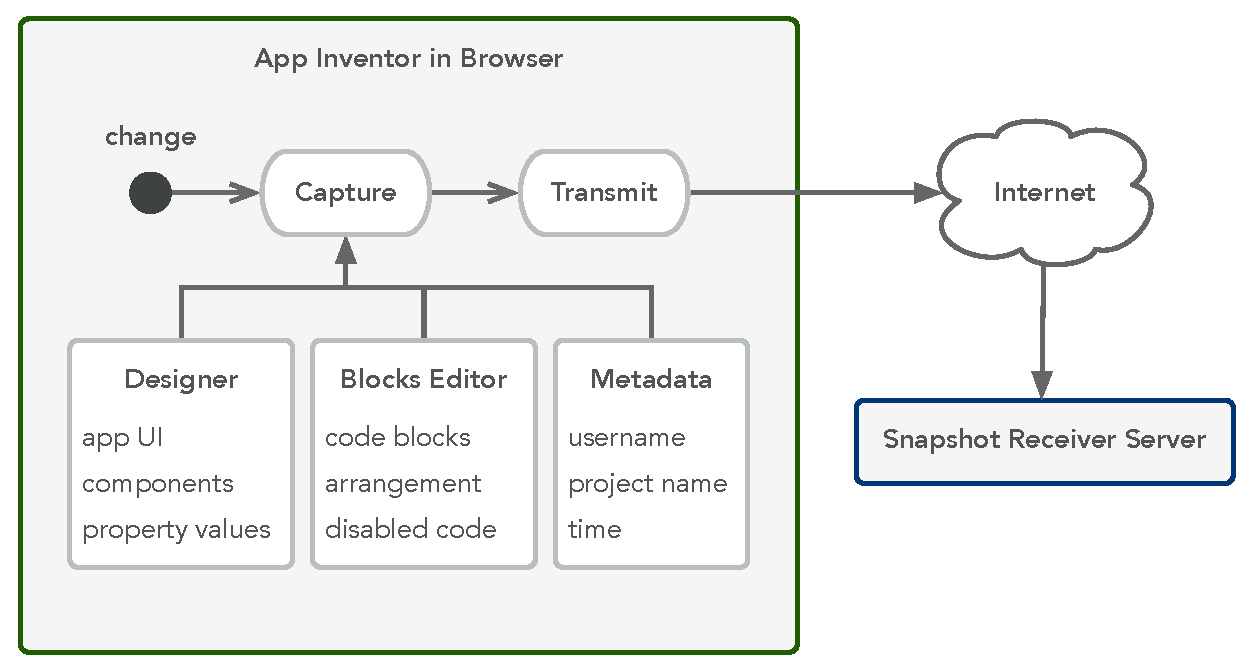
\includegraphics[width=\textwidth]{diagrams/architecture}
  \caption[Snapshot capture design diagram]{The snapshot capture system in App Inventor, which is triggered by any change to blocks or designer. On a change, data from the designer, blocks editor, and additional metadata are captured and transmitted to the receiver server.}
  \label{fig:snapshot-arch}
\end{figure}

The snapshot payload was transmitted upon each user change to a server, where it was de-identified and stored. Details on the server's processes are below, in Section \ref{sec:server}. Additional technical detail on the implementation of the changes to App Inventor are below, in Section \ref{sub:tech:ai}.

\subsection{Snapshot Receiver Server}
\label{sec:server}
The snapshots captured in App Inventor were transmitted to a secure research server, running software that will be described in this section, and called the ``Snapshot Service.'' This server architecture received snapshot payloads from the custom instances of App Inventor, de-identified the user names, and stored the snapshots and metadata persistently. This service had to maintain the integrity of the sensitive, identifiable user data and reliably process peak load, which was tested up to hundreds of snapshots per second. The operation of the server is described in Figure \ref{fig:server-process}


\begin{figure}
  \centering
      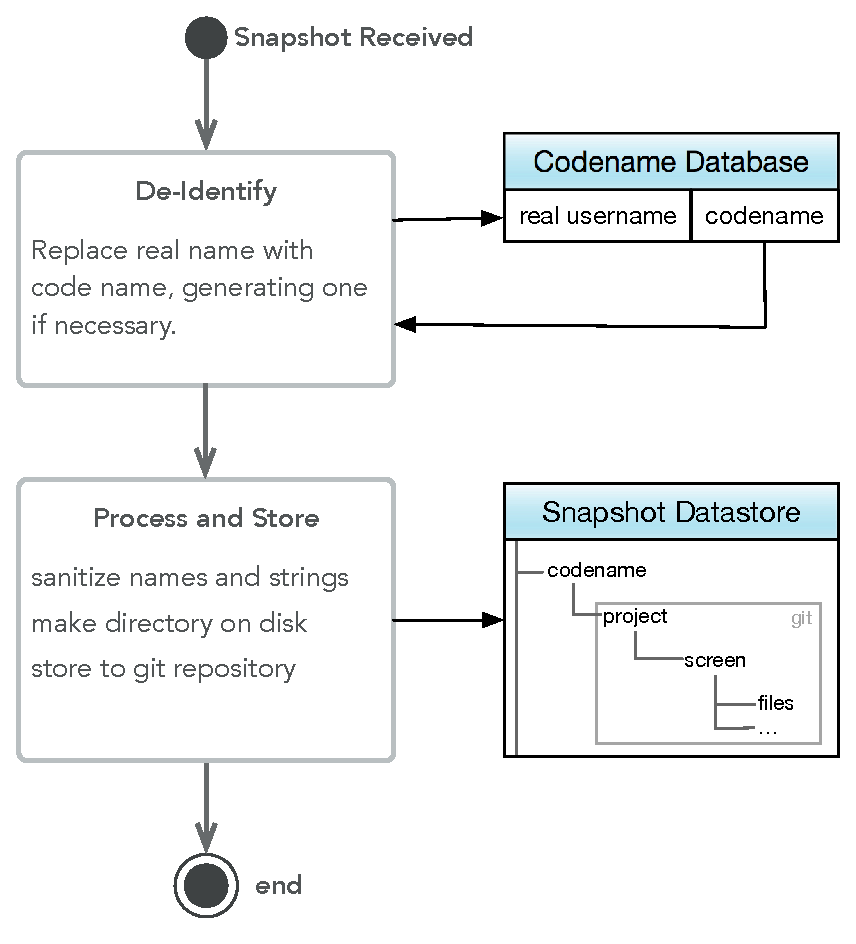
\includegraphics[width=\textwidth]{diagrams/server-operation}
  \caption[Server operating diagram]{Operating diagram for the snapshot collection server. The boxed folder ``project'' denotes the git repository location.}
  \label{fig:server-process}
\end{figure}


\subsection{De-Identification}
\label{sec:deident}
Removal of identifiable user data is a critical issue in human subjects research. In accordance with the IRB approval, student work artifacts had to be stripped of identifiable information, and a system feature was implemented to do so automatically (Appendix \ref{IRB:deident}). This feature replaced the student's real user name with a randomized code name. This feature also kept record of the relations between real names and code names, allowing a consistent mapping. The same user would always be given the same code name, which was critical, as each snapshot was an addition to the data store. Without consistent user-to-code-name mapping, the thousands of snapshots would be like a spilled deck of index cards- useless without order or consistency. 

The map between user names and code names was stored in a database file on the collection server. That server was only accessible to the author, and two trusted IT personnel in the computer science department. Those IT personnel never accessed the server in the time since data collection began. The database selected was sqlite3, because it uses a single, regular file as the data store that could be carefully controlled and protected. That file resided on the server, and was kept separate from the bulk snapshot data. The snapshot data could be moved and analyzed without fear of exposing the real names associated with those data. The mapping database file was only moved off the server in once instance, over encrypted and secured means, to the author's personal computer, which employed a reasonable guarantee of access control, like the server. This protocol was deemed safe by the research team and IRB.

Implementation of the de-identifier was conceptually straightforward- upon every snapshot, look up the user name in the database, and if found, replace the user name with the existing code name. If the user is not in the database, generate a new code name, and insert it into the database. Either way, a code name is returned, and replaces the user name. 

% In the event of an error, the entire snapshot save operation was aborted, so there was no possibility of data being saved without a valid, de-identified code name replacement. The de-identification system was thoroughly tested, protected with regression unit tests, and closely monitored during data collected. During the entire data collection, no error in this system occurred. The combination of sqlite3 and node.js proved to be surprisingly fast, and handled the highest traffic periods with ease. The author would like to attribute this performance in part to their quality and efficient programming, but such cannot be validated scientifically at this time.

% The full source code of the de-identification module is in Appendix \ref{src:userdb.js}.

% \subsection{The Snapshot Database}
% \label{sec:db}
% The database containing the snapshot contents was a collection of git directories. Each user project was a git repository, and each recorded snapshot was a commit into that repository. Additional metadata was included in git notes, or as a content file in the repository. This concept was based on the work of \citet{lipman-phd}. The technology of this database was differentiated by its enhanced granularity of data recorded, adoption of a remote client-server model, and future-looking adapters to allow use of different environments and different languages. The database itself was organized in directories on disk of the server, where the first level of directories contained users. Within each user folder were folders representing each project that was recorded for that user. The project names were a combination of the user-mutable project name and the unique project ID generated by App Inventor. The two fields were concatenated with a \emph{\#} character, which is not allowed in file names and does not occur in project IDs, so it provides a unique token to parse them apart, if needed. Within each project were directories for each screen. Most apps did not extend beyond the default screen, which is always called \emph{Screen1.} Within each screen folder were the contents of the designer and blocks, represented as JSON and XML files, respectively. This is visualized with example data in Table \ref{tab:git-db-org}.

% \begin{table}
% \begin{centering}
% 	\begin{tabular}{ll}
% 	\hline
% 	DB directory&  \mintinline[fontsize=\footnotesize]{bash}{/}		\\
% 	Code name 	&  \mintinline[fontsize=\footnotesize]{bash}{/ColomboMoose}		\\
% 	Project name & \mintinline[fontsize=\footnotesize]{bash}{/ColomboMoose/JumpCount}		\\
% 	Project ID 	&  \mintinline[fontsize=\footnotesize]{bash}{/ColomboMoose/JumpCount#5743573328723968.git}		\\
% 	Screen name	&  \mintinline[fontsize=\footnotesize]{bash}{/ColomboMoose/JumpCount#5743573328723968.git/Screen1}		\\
% 	Blocks code	&  \mintinline[fontsize=\footnotesize]{bash}{/ColomboMoose/JumpCount#5743573328723968.git/Screen1/blocks.xml}		\\
% 	Designer form& \mintinline[fontsize=\footnotesize]{bash}{/ColomboMoose/JumpCount#5743573328723968.git/Screen1/form.json}		\\
% 	\hline
% 	\end{tabular}
% 	\caption[Organization of snapshot database.]{Organization of snapshot database, shown with example data, where each project was a git repository, containing the whole contents of that project's code.}
% 	\label{tab:git-db-org}
% \end{centering}
% \end{table}

% The primary benefit of using git was that it allowed easy human perusal through the time line of projects, and provided code diffs for free. This feature set was briefly useful in assessing that the collection system was working, but in general, these benefits were not highly utilized. Analysis was conducted by developing python scripts to extract features from the data, leaving the human browsing features of git irrelevant. The analysis tools are discussed in depth in Section \ref{sec:analysis-tools}. Additionally, this method of adding many commits to many git repositories is disk-inefficient to git itself, and resulted in an extremely large consumption rate of disk space, and more critically, file system inodes. Disk inodes are the handles that the file system uses to identify and find files, and the maximum number available on an ext4 file system is fixed. Working in this way, git consumed an exorbitant number of these inodes, and required occasional repacking to free them, resulting in the development of the garbage collection script, included in Appendix \ref{src:gc.sh}. While the system was in use, that script needed to be run weekly to prevent the disk from filling and becoming unwritable. 

% \subsection{Engineering Concerns}
% Snapshots captured the entirety of the project's source text at every change. As a program was built, the number of blocks driving it was likely to grow, and the snapshot payload would grow linearly with it. This initially caused concern that the large block files could result in poor performance, such as: slowing down the student's browser, effecting their experience; slow transmission over school networks, creating incomplete or out-of-order snapshot data; or slowdown of the reception server, causing data to be lost or corrupted. In testing, these concerns were allayed. The system performed sufficiently fast under all test cases, indicating that, if possible, a truly extreme case would be necessary to adversely impact performance. The constraints of the experimental design inhibited such massive projects from developing.
% %TODO grab scary concerns from above sections and move them here for better clarity

\section{Technical Detail of Snapshot Collection}

\subsection{Implementation Details of App Inventor Modifications}
\label{sub:tech:ai}
App Inventor was primarily composed using the Google Web Toolkit (GWT), which allows rich web pages to be written in Java and compiled to HTML and javascript. Within the GWT-built App Inventor page there is a panel hosting a somewhat-sandboxed Blockly environment, written in pure javascript. The snapshot mechanism was implemented in the Blockly environment, but required access to certain data in the GWT environment. The interface between GWT and Blockly was implemented in a file \mintinline{js}{BlocklyPanel.java}, which was modified to expose the necessary data. The \mintinline{js}{BlocklyPanel} file was large, with over a thousand lines in length, and governed the entire Blockly sandbox within App Inventor. Exposing new features to Blockly required adding new GWT java methods to extract the data from the GWT-managed memory, and then adding corresponding javascript functions that would be exported into the Blockly environment that serve as wrappers for the GWT methods. Creating new features on this seam between environments was not trivial. %The modifications to this file, but not the file in its entirety, are listed in Appendix \ref{src:ai/BlocklyPanel.java}.

The snapshot mechanism itself was added to Blockly environment, and provided a single external function, \mintinline{js}{Blockly.Snapshot.send}. This function could be called anywhere from within Blockly (or within GWT, with some effort, if desired). In this experiment, snapshots were triggered in only one place, the REPL manager. The REPL manager maintained the connection between App Inventor and the connected target device. When a device was connected, any changes to the app in App Inventor were immediately sent to the device, all while the app continues to run on the device uninterrupted. The REPL manager made this possible, collecting code changes, compiling them, and sending them to the device. The snapshot send function was inserted into the REPL manager's \mintinline{js}{pollYail} routine, which was the function that was called to check if there was a code update to push to the phone. That function was called on-demand by the REPL manager approximately anytime a change was made, with a small amount of change aggregation. That aggregation was intended to service the REPL in a good-enough fashion, which did not require changes to be updated on every pixel-wise change as a block was dragged across the screen, but did require the end position. This function already aggregated trivial, in-motion changes such as block dragging into atomic events, and this degree of granularity was ideal for snapshot capture. 

An alternative trigger point for snapshots was in the \mintinline{js}{blocklyWorkspaceChange} event callback function, but this position was overly aggressive, as it was used in the graphics engine of Blockly to repaint the screen on \emph{any} change. For a snapshot, in-progress block drags across the screen were considered part of the same atomic change. Only the final resting position was necessary for a the desired data density of a snapshot. Additionally, the workspace change event could be called hundreds of time more often than \mintinline{js}{pollYail,} which put unnecessary stress on the snapshot computation and transmission mechanisms. Triggering snapshots from within the REPL manager position, described above, offered an ideal compromise. Every logical block change was captured, but transient state of the block mid-change was not. Additionally, \mintinline{js}{pollYail} was also called in response to changes in the Designer, allowing component changes to trigger snapshots for free.

Another triggering option was considered, where each block type would have the trigger added to their modification callback functions, effectively instrumenting the individual blocks instead of the workspace as a whole. This option could have provided additional specificity, as it could reliably report the nature of the change that triggered the snapshot, such as ``text block was moved.'' The snapshot protocol was designed to accommodate such data, but was not utilized in this study. The engineering demand to implement this style of instrumentation with full coverage was too great to be complete in time for the pilot study. As such, one weakness of the snapshot system as described here is that it does not know why a snapshot was triggered. That was traded for guarantee of full coverage, that no change would be missed. As a result, analysis required the construction of tools to extract that change data from the recorded data. Future work may include such event-driven metadata, and is further explored in Section \ref{sec:futurework}. The snapshot itself contained a collection of fields, shown in Table \ref{tab:snapshotPayload}. 

\begin{table}
\begin{centering}
	\begin{tabular}{l l}
		Data Field 			& Contents \\ \hline
		userName  			& User's real google account name. \\
		projectName 		& User's project file name. 	\\
		projectId 			& Unique ID assigned to the project, invisible to user.	\\
		screenName 			& Which screen in the project the user is modifying.	\\
		sessionId 			& Browser session, to identify session boundaries in analysis.	\\
		yaversion 			& Current version of the App Inventor environment. 	\\
		languageVersion 	& Current version of the App Inventor blocks language. 	\\
		eventType 			& Future use: to explicitly identify the change event that occurred. 	\\
		blocks 				& Full content of the blocks, in XML. 	\\
		form 				& Full content of the screen's design, or form, in JSON.

	\end{tabular}
	\caption[Contents of a snapshot]{The data contents of a single snapshot.}
	\label{tab:snapshotPayload}
\end{centering}
\end{table}

\subsection{Implementation Details of The Collection Server}
The server was written in node.js \citep{nodejs}, a server-side javascript environment that provides high performance and reliability through an event-driven, asynchronous I/O model. %Relevant source code is included in Appendix \ref{src:snapshot-service}.

The service implemented a JSON-RPC API \citep{jsonrpc}, where each snapshot sent from App Inventor was a new RPC connection. There was one API endpoint, which accepted the data, applied the de-identifier, and dispatched the process to commit the change to disk. The RPC API, low-level system access, and git access libraries, were based on similar technology developed by \citet{lipman-2011}. No part of that existing system was used wholesale, but the lessons learned from \citet{lipman-2014} strongly informed the design decisions presented here. Dr. \citeauthor{lipman-2014} also provided code review services for this system. % The logic of the \mintinline{js}{saveProject} process was as follows:

% This is covered in slightly less detail above (better for reading). No need for this degree of specificity.
% \begin{enumerate}
% \item Parse JSON received from App Inventor
% \item Extract real user name from parsed data
% \item Replace real user name with code name (detail below in Section \ref{sec:deident})
% \item Save data to database:
% \begin{enumerate}
% 	\item Sanitize data, removing dangerous dots and slashes from filenames
% 	\item Assemble git commit message
% 	\item Assemble directory for this project based on user code name and project ID
% 	\item Make directory on disk (using -p to only create new as required, preventing overwriting)
% 	\item Write files to directory (blocks and project form)
% 	\item Create git repository in that directory (git re-initializes non-destructively if it already exists)
% 	\item Set git credentials for user, based on code name
% 	\item Stage and commit project files (blocks and project form)
% 	\item Amend current directory as git notes
% \end{enumerate}
% \end{enumerate}


\section{Snapshot Playback}
\label{sec:playback}

A playback system was created to allow researchers to step through the snapshot history of any project. This system afforded the researchers the ability to load the entire history of a particular project, and easily walk through that history. The tool displayed the snapshot number (labeled as ``frame'', like a frame in a video), the time at which the snapshot occurred, and the interval time since the previous interval. 

%To start the playback mechanism, the researcher supplies the \emph{Playback.start} function of the modified version of App Inventor with a file name. The playback module looks for a local web server, fetches that file name, parses the JSON, and returns the control object. 
%The entirety of the module's source code is included in Appendix \ref{src:playback.js}. 
An example of the system at work is shown in Figure \ref{img:playback}. The controls are in the console at the bottom of the screen.

\begin{figure}
  \centering
      \includegraphics[width=\textwidth]{images/ch3-playback}
  \caption[Snapshot playback]{The snapshot playback system in action, showing the final frame of a student project, number 43, which took place at time 16 minutes and 6 seconds, a fair time for the problem. The ``Research Tools'' window contains the snapshot playback controls.}
  \label{img:playback}
\end{figure}
% Note: this image made with data d/AcapulcoDeer





%\section{Assessment}

% The debugging activity, as described above, contained four technical subgoals. There were two artifacts produced, the worksheet, which represented the student's self-report on their performance, and the project file itself, the work product. Both artifacts may not necessarily match, as student's self-report may not be accurate to their real degree of accomplishment. In prior studies, students were incorrect in both directions, self-reporting both above and below the degree of their actual success. 

%To assess these goals across both artifacts, a code set was developed, seen in Tables \ref{tab:debug-worksheet-codes} and \ref{tab:debug-artifact-codes}. % TODO these can probably be reduced into one table with an extra column.



% \begin{table}
% \begin{centering}
% 	\begin{tabular}{lp{13cm}}
% 	\multicolumn{2}{l}{Descriptive (coded as a numeric value)} 	\\ \hline
% 	IN\# 	& Number of bugs correctly identified (can be any of the problems - must be correct problems)	\\
% 	FN\#	& Number of bugs (reportedly) fixed															\\
% 	\\

% 	\multicolumn{2}{l}{Bugs Identified (coded as true or false)} 	\\ \hline
% 	ISK 	& Identified shake response text is wrong.	\\
% 	IS1		& Identified button speak was wrong 1 -- assessed static text as incorrect					\\
% 	IS2		& Identified button speak was wrong 2 -- assessed lack of variable reference to text box		\\
% 	ILL		& Identified updating label with last spoken text												\\
% 	\\

% 	\multicolumn{2}{l}{Bugs Fixed (coded as true or false)} 	\\ \hline
% 	ISK 	& Fixed shake response text is wrong	\\
% 	IS1		& Fixed button speak was wrong 1 -- by changing hard-coded string (or was ambiguous)	\\
% 	IS2		& Fixed button speak was wrong 2 -- by referencing (variable) contents of text box	\\
% 	ILL		& Fixed updating label with last spoken text											\\
% 	\\

% 	\multicolumn{2}{l}{General identification (coded as true or false)} 	\\ \hline
% 	TXT 	& Any mention of text being wrong	\\
% 	VAR		& Any mention of variability of input		\\

% 	\end{tabular}
% 	\caption[Worksheet codes for debugging activity]{Worksheet codes for debugging activity, used when inspecting the worksheet filled out and returned by the student.}
% 	\label{tab:debug-worksheet-codes}
% \end{centering}
% \end{table}

% \begin{table}
% \begin{centering}
% 	\begin{tabular}{lp{13cm}}
% 	\multicolumn{2}{l}{Descriptive (coded as a numeric value)} 	\\ \hline
% 	AN\# 	& Number of bugs attempted (any code change pertaining to it)	\\
% 	CN\#	& Number of bugs (correctly) fixed														\\
% 	\\

% 	\multicolumn{2}{l}{Bugs Attempted (coded as true or false)} 	\\ \hline
% 	ASK 	& Attempt shake response	\\
% 	AS1		& Attempt button speak 1 -- no variable, static text only					\\
% 	AS2		& Attempt button speak 2 -- variable from text box introduced		\\
% 	ALL		& Attempt updating label with last spoken text											\\
% 	\\

% 	\multicolumn{2}{l}{Bugs Fixed (coded as true or false)} 	\\ \hline
% 	CSK 	& Fixed shake response text is wrong	\\
% 	CS1		& Fixed button speak was wrong 1 -- by changing hard-coded string (or was ambiguous)	\\
% 	CS2		& Fixed button speak was wrong 2 -- by referencing (variable) contents of text box	\\
% 	CLL		& Fixed updating label with last spoken text											\\
% 	\\

% 	\multicolumn{2}{l}{General identification (coded as true or false)} 	\\ \hline
% 	CHG 	& Changed blocks in any way	\\

% 	\end{tabular}
% 	\caption[Work artifact codes for debugging activity]{Work artifact codes for the debugging activity, used when inspecting the student's project file.}
% 	\label{tab:debug-artifact-codes}
% \end{centering}
% \end{table}


%\section{Analysis Tools} \label{sec:analysis-tools}



%\chapter{Analysis} 
\chapter{Preliminary Results} % Proposal only
\label{chap:analysis}

Many of the research questions from Section \ref{sec:problem-statement} were answered in this report. The remaining questions require further analysis, which is an ideal position for a dissertation proposal. 

\section{How can a system be built to snapshot blocks-based programming in App Inventor? }
The system is described in detail in Section \ref{sec:mod-ai}.

\section{How can captured snapshot data from ephemeral, remote user sessions be securely and consistently housed in a central server? }
These solutions are described in Sections \ref{sec:server}, \ref{sec:deident}, and \ref{sec:db}.

\section{What is the correct degree of granularity for such snapshot data?}
This blocks-based language provided many options for granularity. The ideal degree for this study was for every notational change to be considered an atom.

\section{What actions by the user in the graphical, blocks-based system are appropriate to trigger a snapshot?}
To capture data with the ideal granularity, snapshots were triggered when a change was completed. This was implemented with good-enough accuracy by App Inventor's REPL manager, as discussed in Section \ref{sec:mod-ai}.

\section{Can data collected by such a system provide clear representations of student progress in a programming work?}
The clarity of the collected data is best justified when viewed in live playback, discussed in Section \ref{sec:playback}, where a researcher can easily walk forwards and backwards through the time line of any collected project history. Viewing data in this wasy immediately provided researchers with a strong model of what the student was experiencing. Analytically, the data has already shown to be rich with extractable features appropriate for data mining.

\section{Particular to App Inventor, how can this data be viewed and replayed to give a viewer a real sense of the work?}
The replay viewer in App Inventor was surprisingly simple to implement, but relied on heavy processing by the analysis software tools to provide the project history in a displayable format. The display mechanism itself leveraged App Inventor's surprising resilience towards the blocks workspace being modified outside of the user's interaction. The system is discussed in detail in Section \ref{sec:playback}.

\section{Are changes in secondary notation (block position and movement) extractable from within snapshot data?}
Yes, changes that affect secondary notation were extractable and differentiable from changes to primary notation.

\section{What other useful measures are extractable from blocks language snapshots?}
So far we have found a few interesting new avenues in these data, including a rich source of interaction with \emph{fields,} any free-form text within the project. Fields can be variable or procedure names, text literals, and other inputs hard-coded by the programmer. Changes to fields were quite prevalent in the data, and may provide further insight.

\section{What techniques would be useful for future blocks instrumentation efforts to improve data efficacy?}
Much of the work of the analysis tools was to reverse engineer what changes occurred from looking at two adjacent snapshots. Future work should avoid this overhead by reporting the conditions of the event triggering the snapshot when it is triggered, so it does not need to be deduced later on. This will be especially important when adapting for real-time detection.

\section{Questions Concerning the Nature of Blocks Programming}
The remaining research questions are still open, and require further analysis. All of the sources of data required have been collected and validated. The tools to access these questions have been built and tested. What remains is to wield these tools in an exploratory analysis to discover what patterns may exist, determine the strength and reliability of these patterns, and optimize the tools to best access those patterns.
\begin{itemize}
\item Can student behavior patterns be detected in snapshot data?
\item Does a pattern of block movement or manipulation exist that signals that the student is not working productively?
\item Can the ratio of secondary notation and formal notation changes indicate anything about the programmer?
\end{itemize}

These questions may be outside the scope of this experiment, and will be reserved for future work:
\begin{itemize}
\item Do the counts of measures, such as secondary notation changes, correlate with other independent variables?
\item Could these patterns and behaviors be detected in real-time?
\end{itemize}

\chapter{Discussion}
	
The change-type features that were extracted from these data would likely be useful in a study where an independent variable describing a behavior of interest could be collected. Such an experiment could be looking for off-task behavior, comparing expert and novice patterns, studying a particular class of common mistake, or any other pattern. With tightly-controlled observations to record the ground truth of the behavior in question, change-type data such as these could be mined against that ground truth to find corresponding relationships. 

A teacher-ready product using particle analysis would consist of a library of solution particle definitions matching activities from the curriculum. The curriculum for App Inventor is largely stable, if varied, and creating solution particle definitions for the most common assignments would benefit teachers active in many different curriculum programs. 

Adding custom definitions of solution particles to match specific activities would require, in its current form, a researcher or developer to design the particles. However, this is not due to the particles being difficult to imagine, but the degree of complexity of the tools with which the particles are currently defined. The elements that make up particles are already defined, abstracted entities that do not require direct manipulation of the underlying blocks representation. One slight exception is the ``close enough'' text comparator, described in Section \ref{sec:close-enough-text}, which was hard-coded with allowable edit distances. It would require a bit more generalization to meet the other elements. But with some wrapping and smoothing, a small language could be developed to express all possibilities of solution particles in a way that would be more accessible to curriculum developers. An even better tool would be able to capture a solution directly from App Inventor and disassemble it into constituent particles automatically. This tool would be the most accessible, and anyone who knows App Inventor to also define canonical solutions for use in the particle analyzer, and with that, the classroom console. 


\section{Detailed Case Analysis}
% overlayed graph with groups of probably-had-intervention and probably-figured--it-outontheir own (temperature activity)
% Temp activity was largey got it or didn't, and if you didn't, you needed an intervention. The debug activity was more continuous.
%
% idea: Statistically identify the "elbow" or corner where graph turns upright, and chart where those happen, and group. 
%		probably a curve-fit to the elbow function, with a parameter - "the logistic function"
%
%TODO here we will go into depth on 2-3 student stories, using:
% notes from Ashley's assessment / mark's distilled codes
% code playback visual to show what they were doing
% particle analysis graphs, matched to code playback
% Tell their stories!


\section{Evaluating the Classroom Console}
% assert console is good, using:
%	Teacher "focus group" feedback
%	Comparison against design goals from literature - Dillenbourg
The researchers recruited a small group of instructors who use App Inventor in their classrooms to see, discuss, and evaluate the Classroom Console. They were interviewed individually, where they were shown the some brief background, the particle assessment concept, a demonstration of the Console. Their reactions were overwhelmingly positive, where the most common question was a form of ``when can I use this?'' The instructors also provided criticism, identified potential weaknesses in the design, and engaged in discussion on how to overcome those weaknesses. One instructor, during the demonstration said, ``I can see right now two students I want to go talk to.'' These discourse are summarized below.

The focus group instructors had two middle school teachers, two middle and high school specialty teachers, two high school and undergraduate instructors, and one undergraduate professor in charge of five lab sections. Their localities included the United States east coast and Midwest, and South America. 

Concerns raised by teachers: 
\begin{itemize}
\item This tool makes it easy to identify high-performing students who can be tasked to help their struggling peers. (Researchers did not realize the tool could be used to identify exemplary performance just as easily as flailing.)
\item Easily identifies ``needy'' students, who ask for help immediately without first trying on their own. %TODO there is definitely a term for this
\item Sometimes you only see students every 8-9 school days, so catching idle periods of mere minutes can be critical. 
\item It is possible for a student who is disengaged to be sitting next to an engaged student, and they both look like they're engaged.
\item When a student returns from a bathroom break, the tool can help assess how quickly they resume engagement.
\item Greatly aids cases where students don't do anything because they know they can get away with it.
\item Training instructors to use the tool may be non-trivial, especially when requiring them to develop their own activities with it. 
\item As the tool is an inexact proxy, experience with the tool may increase the instructor's efficacy with it.
\item High school students are especially afraid to fail, so they often choose not to try anything. This helps identify that behavior.
\item Student feedback often includes the complaint that they did not get enough attention. They could be feeling frustration that the instructor is not seeing, and this helps the instructor gain access into that.
\end{itemize}

Requested Features
\begin{itemize}
\item An automated flag to visually highlight students who are currently exhibiting significant flailing behavior.
\item Flexibility in timeout bar. Some activities and classrooms will have different time frames that would be considered concerning.
\item Treatment for score regression, which is currently not highlighted. 
\item Take the start point with gift code into consideration, and flag the teacher if the student drops below that point, as they have broken their starting configuration and likely need help restoring it.
\item History so teachers can replay or otherwise visual past classroom sessions, and compare them over time. Line chart of the session.
\item HReporting to demonstrate a student's progress in labs over time, suitable for program assessment. 
\item Control over layout, so student locations in Console reflect the seating plan of the classroom.
\item Ability to define your own activities and their corresponding solution particles.
\item Pseudo-anonymized student identifiers, such that the console could be displayed on the projector while the teacher moves around the room.
\end{itemize}

One analysis idea presented by an instructor was to display the \emph{number of attempts} at a certain point of a problem, which would allow the teacher to expect and allow a certain number of attempts before requiring intervention. This method would require further work to better define what an ``attempt'' should mean in general context, and in an activity-specific context.

The instructors were overall excited about the tool, and raised real-world concerns that could further inform the design of the Classroom Console. The instructors declared that the design was ready for prototype use, all citing their desire to use it to enhance their teaching practice.

\section{Conclusions}

%\section{Recommendations} 
% \label{sec:recommendations}
% We do not recommend using git as a database. Further recommendations of legitimate scientific and educational merit will be added as part of the full dissertation.

\section{Future Work}
\label{sec:futurework}

As previously mentioned, there is ample future work to be done in understanding the reasoning behind behavior choices, with particular support to mis-attribution of failure and success. Investigation into this mis-attribution should be conducted, to use traditional methods of assessing student mindset combined with the power of fine-grain snapshot analysis. 

\subsection{Classroom Console and Learning Management Systems}
Different kind of research, but there still is possibility some lit-backed research on how to do this effectively. Take a stab with some lit right here.

\subsection{Towards Programming Skill Assessment}
Someday may have an entire curriculum of activities, and data of kids doing these activities over time. Collected in aggregate for research purposes, could start to isolate skills that are exercised by different activities, and begin to understand how those skills are developing over the course of a curriculum.

\subsection{Solution Particles as Indicators for Further Analysis}
The particle analysis method is, at its core, a feature extractor for snapshot data. For every snapshot, it provides an indicator of progress. That measure of progress has potential to be used to advance real-time classroom tools, and to inform future research. 

One example would be to use solution particle scores as an indicator for same-state. If a student returns to an identical or near-identical state of their code, that student may be experiencing some sort of flailing, in the form of a non-productive iterative behavior. Detecting a return to a previous state is certainly possible from snapshot data, but is potentially computationally expensive. The fast particle scores could serve as a beacon, and could be used as a signal to automatically deploy the more expensive same-state algorithm. The solution scores could reduce the set of possible comparisons for a given snapshot state dramatically, likely allowing it be performed in real-time. This measure could be added to the classroom console or other teacher analytic tool to add richness to the teacher's view of the students' behavior. 
%TODO find some lit references about same-state detection in programming?

The particle score could also be used as a variable for future experiments, and could help to uncover patterns of other properties that correspond with progress made, stalled, or regressed. One such study could take the scores over time in post-hoc data, and encode periods of those histories into states abstract states, describing patterns in the scores, such as flat changes (active non-improvement), fast progress, and regression. These states could be used in in a machine learning experiment to extract correlating patterns in other data, similar to \citet{tissenbaummodeling}, hopefully revealing properties that may be related to those behaviors.

One such design could use a Hidden Markov Model to determine the threshold for automatic flailing detection. This auto-detection could then flag students above threshold in the Classroom Console, further aiding the teacher in deciding where to direct their resources. Inputs to this method would be the particle score graph, or segments of it, with specific measures extracted: interval since last frame, score increase, score decrease, or score the same. 

Further investigation should be given to conditions where students ``win'' at flailing--- when a non-advancing set of changes yields and does not yield advancement. This may be possible with the data from this study. Hypotheses include that flailing/play periods will be different per assignment, and there may be a method, such as the one in the above paragraph, to determine what is reasonable for a particular assignment. 

TODO possible integrity violation detection- it may be possible to use instrumentation to detect the spread of code artifacts physically through the classroom, which could be indicative of integrity, or simply teach us how concepts move through a classroom. Just looking at code playback, there are projects that intuitively ``look like'' they might be engaged in copying solutions. This intuition is based on sudden appearance of code artifacts after somewhat long periods of inactivity. 


\subsection{Better Fine-grain Collection of Snapshot Data} 
In this work, the entire project was captured on every change, which created a need to reverse-engineer what changes occured between snapshots post-facto. Upcoming updates to Blockly will allow for easier access to succinct event descriptions, potentially allowing only the changes themselves to be sent, effectively reducing the transmission payload and increasing transparency of collected data. Such improvements can make future collection experiments easier, and provide data that is richer for analysis, with no loss in accuracy. 

\subsection{Novice and Expert Behaviors}
There is also work to be done in assessing expert and novice usage patterns using snapshot analysis. \cite{petre-1995} outlined a strong difference in reading and authoring skills pertaining to secondary notation between expert and novice users. Teaching App Inventor, like any language, includes showing patterns that are good standards of practice, in hopes of the student developing more expert skills. Those patterns are not yet based on scientific observation of expert and novice programming behaviors. Snapshot analysis may be critical to provide insight into expert patterns, which could then be disseminated to enhance teaching practice. 


\include{bibliography}
\appendix
\chapter{Institutional Compliance Forms}
This project was monitored by the UMass Lowell Office of Institutional Compliance Institutional Review Board (IRB). This section contains the relevant submissions and approval letters between the research team and the IRB.

\section{IRB Application}
\label{IRB:app}
"Middle School Pathways in Computer Science" was originally submitted by Fred Martin on June 25, 2014. Approval was received after expedited review on July 7, 2014, as IRB Protocol \# 14-144-MAR-XPD. The approval period was for July 7, 2014 through July 6, 2015.

The following pages contain a copy of the IRB application form and the approval letter in response.

\includepdf[pages=-]{IRB/14-144-app.pdf}
\includepdf[pages=-]{IRB/14-144-apv.pdf}

\section{Debugging Activity}
This amendment added the author, Mark Sherman, and fellow researcher Lijun Ni to the project. This amendment also specified the Debugging Activity, and its protocol for classroom use, which was used in this experiment. The Debugging Activity included the data de-identification protocol. Additionally, this amendment specified a structured interview protocol and updated a summer camp student survey, neither of which where used for this research and have been excluded from this document.

The following pages contain a copy of the amendment application, the approval letter, and the included Debugging Activity protocol, which includes the data de-identification protocol specification used in this project, as described in Section \ref{sec:deident}.

\includepdf[pages=-]{IRB/AM2-application.pdf}
\includepdf[pages=-]{IRB/AM2-approve.pdf}
\label{IRB:deident}
\includepdf[pages=-]{IRB/AM2-DebuggingActivity2015.pdf}
%TODO maybe break into sections, so the debugging activity protocol has a subsection (it has the de-ident protocol)

\section{Annual/Continuing Review 2015}
This application updated the IRB on the activities of the first year of the grant project, and declared intent for ongoing participant recruitment and data analysis until August 31, 2017. The following pages contain a copy of the review application and approval letter. The letter also mentions Amendment 3, which was approved at the same time, but is not relevant to the research in this document.

\includepdf[pages=-]{IRB/Year1-review-apl.pdf}
\includepdf[pages=-]{IRB/Year1-review-apv.pdf}

\section{Informed Consent, In-School}
\label{sec:icf:school}
The participants in this study were children, so an informed consent form was created for their parents, and a student assent form was provided to the children. The following pages are copies of those consent and assent forms as they were presented to the in-school cohort.
\includepdf[pages=-]{IRB/icf-parent-in-school-rev3-9-14-15.pdf}
\includepdf[pages=-]{IRB/icf-assent-8-21-15.pdf}


\section{Informed Consent, Summer Camp}
\label{sec:icf:camp}
The participants in this study were children, so an informed consent form was created for their parents, and a student assent form was provided to the children. The student assent form was unchanged from the In-School cohort (Appendix \ref{sec:icf-school}). The parental consent form was updated. The following pages are copies of the updated summer camp parental consent and the corresponding IRB approval letter.

\includepdf[pages=-]{IRB/icf-summer-camp-parent-consent-2016.pdf}
\includepdf[pages=-]{IRB/icf-summer-camp-parent-consent-2016-approval.pdf}


\section{Student Activities for this Research}
Amendment 10 added protocols for the Debugging Activity and Temperature Activity, both of which were used for data collection in this research. The protocol documents follow in Sections \ref{sec:IRB:debugging} and \ref{sec:IRB:temperature}, respectively. The following pages are copies of the IRB amendment form, and the approval letter affirming that these instruments operate under previously approved informed consent mechanisms. 

\includepdf[pages=-]{IRB/AM10-application.pdf}
\includepdf[pages=-]{IRB/AM10-apv.pdf}


\section{Debugging Activity Protocol}
\includepdf[pages=-]{IRB/AM10DebuggingAssessment.pdf}
\label{sec:IRB:debugging}


\section{Temperature Activity Protocol}
\includepdf[pages=-]{IRB/AM10TemperatureAssessment.pdf}
\label{sec:IRB:temperature}


%%%%%%%%%%%%%%%%%%%%%%%%%%%%%%%%%%%%%%%%%%%%%%%%%%%%%%%%%%%%%%%%%%%%%%%%%%%%%%%%
%%%%%%%%%%%%%%%%%%%%%%%%%%%%%%%%%%%%%%%%%%%%%%%%%%%%%%%%%%%%%%%%%%%%%%%%%%%%%%%%


\chapter{Code Listings}
Source code for the data capture, collection, and analysis systems used in this project are listed in full here. All code was written by the author except where noted.

% font sizes, ascending: \tiny \scriptsize \footnotesize \small \normalsize
% scriptsize gets a little more than 80 chars wide and 44 lines on the page, which is fair.
\setminted{fontsize=\scriptsize, fontfamily=courier, linenos, breaklines}

\section{Modifications to App Inventor}
\label{src:appinventor}

\subsection{snapshot.js}
\label{src:ai/snapshot.js}
This file was added to the blockly editor within App Inventor, and provided the snapshot collection and transmission features. The public function is \emph{Blockly.Snapshot.send,} which was called elsewhere in blockly to trigger a snapshot. As listed below, the feature will connect to a local test server. For production, the comments on line 13 and 14 were swapped, allowing connection to the real data collection server. 
\inputminted{javascript}{src/appinventor/snapshot.js}

\subsection{Modifications to BlocklyPanel.java}
\label{src:ai/BlocklyPanel.java}
This file provided the interface between the general App Inventor web page, including the Designer, and the javascript blockly environments. The page and Designer were composed using the Google Web Toolkit (GWT), which was written in Java and compiled to javascript. The snapshot mechanism was implemented in the blockly environment, in pure javascript, but required access to certain data in the GWT environment. Modifications to this file exposed that data to blockly, and the snapshot system, as seen in the file excerpts below.

\inputminted[firstline=626, lastline=651]{java}{src/appinventor/BlocklyPanel.java}
\inputminted[firstline=902, lastline=913, breakbefore=.]{java}{src/appinventor/BlocklyPanel.java}

\section{Snapshot Service}
\label{src:snapshot-service}
The Snapshot Service was the server-side receiving mechanism that de-identified and stored snapshots generated by App Inventor. This service was written in javascript for node.js.

\subsection{file.js}
\label{src:file.js}
RPC module that implements the \emph{file.saveProject} API endpoint. It takes raw snapshot data, applies the de-identifier, and saves the snapshot to disk.
\inputminted{javascript}{src/snapshot-service/file.js}

\subsection{userdb.js}
\label{src:userdb.js}
De-identifies user names, replacing them with unique code names, and stores the relationship in a database.
\inputminted{javascript}{src/snapshot-service/userdb.js}

\subsection{savegit.js}
\label{src:savegit.js}
Provides utilities to interface with git on the server to save data. Each user's project is represented by a git repository, and each snapshot creates a new commit in that repository. This is used by file.js.
\inputminted{javascript}{src/snapshot-service/savegit.js}

\subsection{gc.sh}
\label{src:gc.sh}
The additive git method used by this service creates inefficiencies on the host file system that consumes space and inodes at a high rate. This script `garbage collects' the database, repacking it efficiently, and should be run occasionally while the system is in use. This file is included here as a warning to anyone in the future who wants to use git as a database.
\inputminted{bash}{src/snapshot-service/gc.sh}
\chapter{Code Listing Excerpts} \label{appendix:listings}

Interesting source code for the data capture, collection, and analysis systems used in this project are listed here. 

% font sizes, ascending: \tiny \scriptsize \footnotesize \small \normalsize
% scriptsize gets a little more than 80 chars wide and 44 lines on the page, which is fair.
\setminted{fontsize=\scriptsize, fontfamily=courier, linenos, breaklines}

% CHAPTER 4
\section{Field Change Accumulator}
\label{src:reduceFieldChanges}

\begin{listing}[]
\begin{minted}{python}
def reduceFieldChanges(changes):
    """Reduces char-by-char field changes into a single change.
    Operates on a list of changes, and modifies that list in place.
    This would run on the return value from processProject.
    Returns nothing, as changes are made in the passed-in structure itself.
    Identifies changes to the same field, and reduces them to their final state.
    Also has a 10-second timeout window, so changes 10 seconds apart are kept.
    """

    changesToDelete = []
    prevFlag = False
    prevList = []
    prevChange = {'date': '0'}
    prevTime = 0

    for thisChange in changes:
        thisFlag = False
        thisList = []
        thisTime = thisChange.get('seconds_elapsed')
        features = []

        # if a field changed in this change, take the list of all field changed blocks 
        # and add to list
        if thisChange.get(names.featureExtractionResults):
            features = thisChange[names.featureExtractionResults]
            thisFlag = features[names.blocksFieldsChangedFlag]
        if thisFlag:
            thisList = features[names.blocksFieldsChangedList]

        # Identify blocks from this change and the prev change whose fields were modified
        # Include those blocks for deletion UNLESS they're more than 10 seconds apart
        # remember empty lists are falsey!
        deleteMe = prevFlag and thisFlag
        deleteMe = deleteMe and intersect(prevList, thisList)
        deleteMe = deleteMe and (thisTime - prevTime < 10)

        if deleteMe:
            changesToDelete.append(prevChange)

        prevFlag = thisFlag
        prevList = thisList
        prevChange = thisChange
        prevTime = thisTime

    for c in changesToDelete:
        changes.remove(c)
\end{minted}
\caption{The Field Change Accumulator}
\label{src:lst:field-change}
\end{listing}

Listing \ref{src:lst:field-change} presents the code used for the text field change accumulator described in Section \ref{sec:text-acc}. This algorithm operated on a single project, represented as a list of changes in historical order. It identified when the a text field was modified multiple times in rapid succession and reduced that series of changes to its final state.

This algorithm was part of the post-hoc analysis tools, and was not part of the real-time assessment algorithm.


\section{Feature Extraction Tests}
\label{src:feature-extraction-tests}

Below are the code listings for the feature extraction module, as discussed in Section \ref{sec:feature-extraction}, displayed as Listings \ref{src:lst:add-delete}--\ref{src:lst:properties-modified}. All of these tests took representations of two adjacent snapshots as arguments. Data types representing snapshots could be any of the following: ``root,'' which was the tree structures of the blocks itself; ``IDmap,'' a structure mapping ID numbers to blocks; or ``parentMap,'' a structure mapping block ID numbers to their parent blocks. There were also helper functions to access and manipulate these structures, whose definitions are unneccesary to understand their function, and were not included here.

All of these tests returned an array containing references to the blocks for which the test was true. Returning an empty array indicated that no blocks were found, and that specific change type did not occur between the two given snapshots.

Helper functions have been included here where they were necessary to fully understand the operation of the test. These tests were written in python and made significant use of list comprehensions \citep{oliphant2007python}.

\begin{listing}[]
\begin{minted}{python}
def checkForDeletedAddedBlocks(rootA, rootB):
    """Returns lists: deleted and added blocks from A to B."""
    iterA = rootA.iter(BLOCK)
    iterB = rootB.iter(BLOCK)
    setA = frozenset([el.get('id') for el in iterA])
    setB = frozenset([el.get('id') for el in iterB])
    deleted = setA.difference(setB)
    added = setB.difference(setA)
    return list(deleted), list(added)
\end{minted}
\caption{Test for Added and/or Deleted Blocks}
\label{src:lst:add-delete}
\end{listing}

\begin{listing}[]
\begin{minted}{python}
def checkForMovedBlocks(IDmapA, IDmapB):
    """Returns list: blocks that moved in space or context from A to B."""
    # only check blocks that exist in both time steps (set intersection)
    blockIDs = commonKeys(IDmapA, IDmapB)
    return [i for i in blockIDs if didThisBlockMoveinSpace(IDmapA[i], IDmapB[i])]

# Returns
#   True: block is top-level and moved on workpace
#   False: block was moved in or out of top-level (in/out of being nested)
#   False: block is top level and coordinates did not change
#   False: block is nested and stayed as such (though parent may have moved)
def didThisBlockMoveinSpace(blockA, blockB):
    """Checks the same block element at two different times for motion in space"""
    sameBlockCheck(blockA, blockB)
    # isTop* is True if location coordinates are in that block
    isTopA = isBlockTopLevel(blockA)
    isTopB = isBlockTopLevel(blockB)

    if isTopA and isTopB:
        # both are top-level
        return blockA.get('x') != blockB.get('x') or blockA.get('y') != blockB.get('y')
    else:
        # block either is not top level or changed contexts
        return False
\end{minted}
\caption{Test for Moved Blocks (on workspace)}
\end{listing}

\begin{listing}[]
\begin{minted}{python}
def checkForContextMove(IDmapA, IDmapB, parentMapA, parentMapB):
    """Returns list: blocks that moved in context, having a new parent, from A to B"""
    blockIDs = commonKeys(IDmapA, IDmapB)
    # for each ID, get that block, and compare parentmaps
    return [i for i in blockIDs if
            findParentBlockByID(i, parentMapA, IDmapA).get('id') !=
            findParentBlockByID(i, parentMapB, IDmapB).get('id')]
\end{minted}
\caption{Test for Blocks Moving in Context}
\end{listing}

\begin{listing}[]
\begin{minted}{python}
def checkForFieldChanges(IDmapA, IDmapB):
    """Returns list: blocks whose field(s) changed from A to B, common to A&B"""
    blockIDs = commonKeys(IDmapA, IDmapB)
    return [i for i in blockIDs if didThisBlocksFieldsChange(IDmapA[i], IDmapB[i])]

def didThisBlocksFieldsChange(blockA, blockB):
    """Detect text field changes, whether strings or variable names, etc"""
    fieldsA = blockA.findall(ns + 'field')
    fieldsB = blockB.findall(ns + 'field')
    for fA, fB in zip(fieldsA, fieldsB):
        if fA.text != fB.text:
            return True
    return False
\end{minted}
\caption{Test for Text Field Changes}
\end{listing}

\begin{listing}[]
\begin{minted}{python}
def checkForChangedBlocks(IDmapA, IDmapB):
    """Returns list: blocks that changed (not moved) from A to B, common to A&B"""
    blockIDs = commonKeys(IDmapA, IDmapB)
    return [i for i in blockIDs if didThisBlockChange(IDmapA[i], IDmapB[i])]

def didThisBlockChange(blockA, blockB):
    """True: blockA/B and their child Elements DIFFER, ignoring fields."""
    sameBlockCheck(blockA, blockB)

    # ElementEqual ignores x/y by default
    if not ElementEqual(blockA, blockB):
        return True

    # This assumes blocks cannot be direct descendants of other blocks-
    #   which seems to be true as blocks must be plugged into a value socket.
    #   As a result, no filtering for non-block children is performed
    childrenA = [e for e in blockA.findall('*') if e.tag != ns + 'field']
    childrenB = [e for e in blockB.findall('*') if e.tag != ns + 'field']

    if len(childrenA) != len(childrenB):
        return True

    for childA, childB in zip(childrenA, childrenB):
        if not ElementEqual(childA, childB):
            return True

    # passed all tests without finding a change, so it must not have changed.
    return False
\end{minted}
\caption{Test for Properties Modified}
\label{src:lst:properties-modified}
\end{listing}

%%%%% Whole-file code listings from early version of the proposal. %%%%%

% \section{Modifications to App Inventor}
% \label{src:appinventor}

% \subsection{snapshot.js}
% \label{src:ai/snapshot.js}
% This file was added to the blockly editor within App Inventor, and provided the snapshot collection and transmission features. The public function is \emph{Blockly.Snapshot.send,} which was called elsewhere in blockly to trigger a snapshot. As listed below, the feature will connect to a local test server. For production, the comments on line 13 and 14 were swapped, allowing connection to the real data collection server. 
% \inputminted{javascript}{src/appinventor/snapshot.js}

% \subsection{Modifications to BlocklyPanel.java}
% \label{src:ai/BlocklyPanel.java}
% This file provided the interface between the general App Inventor web page, including the Designer, and the javascript blockly environments. The page and Designer were composed using the Google Web Toolkit (GWT), which was written in Java and compiled to javascript. The snapshot mechanism was implemented in the blockly environment, in pure javascript, but required access to certain data in the GWT environment. Modifications to this file exposed that data to blockly, and the snapshot system, as seen in the file excerpts below.

% \inputminted[firstline=626, lastline=651]{java}{src/appinventor/BlocklyPanel.java}
% \inputminted[firstline=902, lastline=913, breakbefore=.]{java}{src/appinventor/BlocklyPanel.java}


% \section{Snapshot Receiver Service}
% \label{src:snapshot-service}
% The Snapshot Service was the server-side receiving mechanism that de-identified and stored snapshots generated by App Inventor. This service was written in javascript for node.js.

% \subsection{file.js}
% \label{src:file.js}
% RPC module that implements the \emph{file.saveProject} API endpoint. It takes raw snapshot data, applies the de-identifier, and saves the snapshot to disk.
% \inputminted{javascript}{src/snapshot-service/file.js}

% \subsection{userdb.js}
% \label{src:userdb.js}
% De-identifies user names, replacing them with unique code names, and stores the relationship in a database.
% \inputminted{javascript}{src/snapshot-service/userdb.js}

% \subsection{savegit.js}
% \label{src:savegit.js}
% Provides utilities to interface with git on the server to save data. Each user's project is represented by a git repository, and each snapshot creates a new commit in that repository. This is used by file.js.
% \inputminted{javascript}{src/snapshot-service/savegit.js}

% \subsection{gc.sh}
% \label{src:gc.sh}
% The additive git method used by this service creates inefficiencies on the host file system that consumes space and inodes at a high rate. This script `garbage collects' the database, repacking it efficiently, and should be run occasionally while the system is in use. This file is included here as a warning to anyone in the future who wants to use git as a database.
% \inputminted{bash}{src/snapshot-service/gc.sh}


% \section{Analysis Tools}

% \subsection{main.py}
% %TODO This needs to be updated when the scrips change! Make sure this is re-copied latex directory before final thesis print!
% This is currently an in-progress version of this file, containing provisional scratchwork and some in-development modifications. These temporary features will be removed and replaced with restored, fully consistent code for the final dissertation document.
% \inputminted[lastline=212]{python}{src/analysis/main.py}

% \subsection{gitfilter.py}
% \inputminted[lastline=168]{python}{src/analysis/gitfilter.py}
% \subsection{xml\_analyze.py}
% \inputminted[lastline=261]{python}{src/analysis/xml_analyze.py}


% \section{Snapshot Playback}
% The playback mechanism allowed a full history of snapshots from a project to be viewed in an App Inventor blockly window. It enabled the researcher to step through the history- forward, backwards, and arbitrarily, displaying the code blocks as the user placed them. Additionally the mechanism displayed the timestamp of the current snapshot, in seconds since the project was created, how many snapshots were taken, and what number snapshot was currently being viewed.

% This file, \emph{playback.js,} was added to the blockly editor within App Inventor, and provided the playback feature. It used the javascript console to start and control playback.
% \label{src:playback.js}
% \inputminted{javascript}{src/playback/playback.js}
\chapter{Author Biography}

Mark Sherman attended University of Massachusetts Lowell, earning a  Bachelor of Science degree in Computer \& Electrical Engineering, in 2008, demonstrating a capstone project in capacitive touchscreen technology. He continued his studies at UMass~Lowell, moving to the Computer Science department, and earned a Master of Science degree in Computer Science in 2010, with a research focus in computer science education. His masters thesis ``Exploration of Natural Design Tendencies of Novice Engineers'' identified testing and iteration patterns that may contribute to successful completion of engineering puzzles.

Mark is a proud member of the UMass Lowell Engaging Computing Group, where he has worked since 2008.

Mark also serves as an App Inventor Master Trainer with MIT, where he visits winning teams of a national design competition, trains students and teachers in App Inventor, programming, and project management to facilitate the teams production of a functional mobile application.
Projects mentored:
\begin{itemize}
\item HeadTek: Hardware and software solution for recording and processing head impact data with real-time data
reporting to mobile devices. Suitable for football, bike riding, and other impact-wary activities. Arduino, Firebase noSQL cloud database, sensors, real-time data, mobile visualization. Pine Crest Middle School, Fort Lauderdale, FL, 2016.
\item A Look Inside: App to explore inner workings of everyday devices. Provided clickable images that zoom into subcomponents with explanatory text. Utilized cloud SQL database to provide updatable list of devices, images, text, maps of click zones, traversal maps. FusionTables database, 3D modeling, custom data parser design. Upper St. Clair High School, Pittsburgh, PA, 2015.
\item SnapDocs: Utilize cloud-based optical character recognition from document scanner app, provide text representation of image. Cheney Middle School, Fargo, ND, 2014.
\item ChowChecker: Search for foods and display allergens present. Utilized online food databases and parsed ingredients lists. Hampstead Academy High School, Hampstead, NH, 2013.
\item Recycle Bin: Identified nearby recycling centers, helped community members form new recycling initiatives. STEM Center Middle School, Fargo, ND, 2013
\end{itemize}

\noindent Undergraduate courses at UMass Lowell: Organization of Programming Languages, Computing I, and Exploring the Internet.

\noindent Workshops developed and/or instructed: CAITE professional development for App Inventor; UMass Lowell Summer Bridge program; MassBay Community College Summer Bridge program; Beauty \& Joy of Computing professional development; Introduction to Mobile Robotics for Professors at Chitkara University, Chandigarh, India; undergraduate intensive in Mobile Robotics in Guangzou, China. 



\end{document}
